% Options for packages loaded elsewhere
\PassOptionsToPackage{unicode}{hyperref}
\PassOptionsToPackage{hyphens}{url}
%
\documentclass[
  12pt,
]{article}
\usepackage{amsmath,amssymb}
\usepackage{iftex}
\ifPDFTeX
  \usepackage[T1]{fontenc}
  \usepackage[utf8]{inputenc}
  \usepackage{textcomp} % provide euro and other symbols
\else % if luatex or xetex
  \usepackage{unicode-math} % this also loads fontspec
  \defaultfontfeatures{Scale=MatchLowercase}
  \defaultfontfeatures[\rmfamily]{Ligatures=TeX,Scale=1}
\fi
\usepackage{lmodern}
\ifPDFTeX\else
  % xetex/luatex font selection
\fi
% Use upquote if available, for straight quotes in verbatim environments
\IfFileExists{upquote.sty}{\usepackage{upquote}}{}
\IfFileExists{microtype.sty}{% use microtype if available
  \usepackage[]{microtype}
  \UseMicrotypeSet[protrusion]{basicmath} % disable protrusion for tt fonts
}{}
\makeatletter
\@ifundefined{KOMAClassName}{% if non-KOMA class
  \IfFileExists{parskip.sty}{%
    \usepackage{parskip}
  }{% else
    \setlength{\parindent}{0pt}
    \setlength{\parskip}{6pt plus 2pt minus 1pt}}
}{% if KOMA class
  \KOMAoptions{parskip=half}}
\makeatother
\usepackage{xcolor}
\usepackage[margin=1in]{geometry}
\usepackage{color}
\usepackage{fancyvrb}
\newcommand{\VerbBar}{|}
\newcommand{\VERB}{\Verb[commandchars=\\\{\}]}
\DefineVerbatimEnvironment{Highlighting}{Verbatim}{commandchars=\\\{\}}
% Add ',fontsize=\small' for more characters per line
\usepackage{framed}
\definecolor{shadecolor}{RGB}{248,248,248}
\newenvironment{Shaded}{\begin{snugshade}}{\end{snugshade}}
\newcommand{\AlertTok}[1]{\textcolor[rgb]{0.94,0.16,0.16}{#1}}
\newcommand{\AnnotationTok}[1]{\textcolor[rgb]{0.56,0.35,0.01}{\textbf{\textit{#1}}}}
\newcommand{\AttributeTok}[1]{\textcolor[rgb]{0.13,0.29,0.53}{#1}}
\newcommand{\BaseNTok}[1]{\textcolor[rgb]{0.00,0.00,0.81}{#1}}
\newcommand{\BuiltInTok}[1]{#1}
\newcommand{\CharTok}[1]{\textcolor[rgb]{0.31,0.60,0.02}{#1}}
\newcommand{\CommentTok}[1]{\textcolor[rgb]{0.56,0.35,0.01}{\textit{#1}}}
\newcommand{\CommentVarTok}[1]{\textcolor[rgb]{0.56,0.35,0.01}{\textbf{\textit{#1}}}}
\newcommand{\ConstantTok}[1]{\textcolor[rgb]{0.56,0.35,0.01}{#1}}
\newcommand{\ControlFlowTok}[1]{\textcolor[rgb]{0.13,0.29,0.53}{\textbf{#1}}}
\newcommand{\DataTypeTok}[1]{\textcolor[rgb]{0.13,0.29,0.53}{#1}}
\newcommand{\DecValTok}[1]{\textcolor[rgb]{0.00,0.00,0.81}{#1}}
\newcommand{\DocumentationTok}[1]{\textcolor[rgb]{0.56,0.35,0.01}{\textbf{\textit{#1}}}}
\newcommand{\ErrorTok}[1]{\textcolor[rgb]{0.64,0.00,0.00}{\textbf{#1}}}
\newcommand{\ExtensionTok}[1]{#1}
\newcommand{\FloatTok}[1]{\textcolor[rgb]{0.00,0.00,0.81}{#1}}
\newcommand{\FunctionTok}[1]{\textcolor[rgb]{0.13,0.29,0.53}{\textbf{#1}}}
\newcommand{\ImportTok}[1]{#1}
\newcommand{\InformationTok}[1]{\textcolor[rgb]{0.56,0.35,0.01}{\textbf{\textit{#1}}}}
\newcommand{\KeywordTok}[1]{\textcolor[rgb]{0.13,0.29,0.53}{\textbf{#1}}}
\newcommand{\NormalTok}[1]{#1}
\newcommand{\OperatorTok}[1]{\textcolor[rgb]{0.81,0.36,0.00}{\textbf{#1}}}
\newcommand{\OtherTok}[1]{\textcolor[rgb]{0.56,0.35,0.01}{#1}}
\newcommand{\PreprocessorTok}[1]{\textcolor[rgb]{0.56,0.35,0.01}{\textit{#1}}}
\newcommand{\RegionMarkerTok}[1]{#1}
\newcommand{\SpecialCharTok}[1]{\textcolor[rgb]{0.81,0.36,0.00}{\textbf{#1}}}
\newcommand{\SpecialStringTok}[1]{\textcolor[rgb]{0.31,0.60,0.02}{#1}}
\newcommand{\StringTok}[1]{\textcolor[rgb]{0.31,0.60,0.02}{#1}}
\newcommand{\VariableTok}[1]{\textcolor[rgb]{0.00,0.00,0.00}{#1}}
\newcommand{\VerbatimStringTok}[1]{\textcolor[rgb]{0.31,0.60,0.02}{#1}}
\newcommand{\WarningTok}[1]{\textcolor[rgb]{0.56,0.35,0.01}{\textbf{\textit{#1}}}}
\usepackage{graphicx}
\makeatletter
\def\maxwidth{\ifdim\Gin@nat@width>\linewidth\linewidth\else\Gin@nat@width\fi}
\def\maxheight{\ifdim\Gin@nat@height>\textheight\textheight\else\Gin@nat@height\fi}
\makeatother
% Scale images if necessary, so that they will not overflow the page
% margins by default, and it is still possible to overwrite the defaults
% using explicit options in \includegraphics[width, height, ...]{}
\setkeys{Gin}{width=\maxwidth,height=\maxheight,keepaspectratio}
% Set default figure placement to htbp
\makeatletter
\def\fps@figure{htbp}
\makeatother
\setlength{\emergencystretch}{3em} % prevent overfull lines
\providecommand{\tightlist}{%
  \setlength{\itemsep}{0pt}\setlength{\parskip}{0pt}}
\setcounter{secnumdepth}{-\maxdimen} % remove section numbering
% definitions for citeproc citations
\NewDocumentCommand\citeproctext{}{}
\NewDocumentCommand\citeproc{mm}{%
  \begingroup\def\citeproctext{#2}\cite{#1}\endgroup}
\makeatletter
 % allow citations to break across lines
 \let\@cite@ofmt\@firstofone
 % avoid brackets around text for \cite:
 \def\@biblabel#1{}
 \def\@cite#1#2{{#1\if@tempswa , #2\fi}}
\makeatother
\newlength{\cslhangindent}
\setlength{\cslhangindent}{1.5em}
\newlength{\csllabelwidth}
\setlength{\csllabelwidth}{3em}
\newenvironment{CSLReferences}[2] % #1 hanging-indent, #2 entry-spacing
 {\begin{list}{}{%
  \setlength{\itemindent}{0pt}
  \setlength{\leftmargin}{0pt}
  \setlength{\parsep}{0pt}
  % turn on hanging indent if param 1 is 1
  \ifodd #1
   \setlength{\leftmargin}{\cslhangindent}
   \setlength{\itemindent}{-1\cslhangindent}
  \fi
  % set entry spacing
  \setlength{\itemsep}{#2\baselineskip}}}
 {\end{list}}
\usepackage{calc}
\newcommand{\CSLBlock}[1]{\hfill\break\parbox[t]{\linewidth}{\strut\ignorespaces#1\strut}}
\newcommand{\CSLLeftMargin}[1]{\parbox[t]{\csllabelwidth}{\strut#1\strut}}
\newcommand{\CSLRightInline}[1]{\parbox[t]{\linewidth - \csllabelwidth}{\strut#1\strut}}
\newcommand{\CSLIndent}[1]{\hspace{\cslhangindent}#1}
\usepackage{geometry}
\geometry{left=1in, right=1in, top=1in, bottom=1in}
\setlength{\textwidth}{6in}
\usepackage{setspace}
\onehalfspacing
\usepackage{titlesec}
\titleformat{\section}[block]{\normalfont\Large\bfseries\centering}{\thesection}{1em}{}
\usepackage{fancyhdr}
\pagestyle{fancy}
\setlength{\headheight}{15pt}
\fancyhead[L]{}
\fancyhead[C]{Template RMarkdown File}
\fancyhead[R]{}
\fancyfoot[L]{}
\fancyfoot[C]{\thepage}
\fancyfoot[R]{}
\usepackage{hyperref}
\usepackage{amsmath}
\usepackage{amsfonts}
\usepackage{amssymb}
\usepackage{enumitem}
\usepackage{microtype}
\usepackage{fvextra}
\usepackage{fontspec}
\setmainfont{Times New Roman}
\setsansfont{Arial}
\setmonofont{Source Code Pro}
\ifLuaTeX
  \usepackage{selnolig}  % disable illegal ligatures
\fi
\usepackage{bookmark}
\IfFileExists{xurl.sty}{\usepackage{xurl}}{} % add URL line breaks if available
\urlstyle{same}
\hypersetup{
  pdftitle={Template RMarkdown File},
  pdfauthor={Robert J. Dellinger},
  hidelinks,
  pdfcreator={LaTeX via pandoc}}

\title{Template RMarkdown File}
\author{Robert J. Dellinger}
\date{April 06, 2025}

\begin{document}
\maketitle

{
\setcounter{tocdepth}{3}
\tableofcontents
}
\newpage

\section{Introduction}\label{introduction}

This document outlines the methodology for data cleaning, exploration,
and visualization. It is structured to ensure transparency and
reproducibility of all analyses.

\subsection{Methodology}\label{methodology}

Briefly describe the methods used in the project, including data
sources, cleaning steps, and techniques applied to handle missing or
inconsistent data.

\subsubsection{Math Equations with
LaTeX}\label{math-equations-with-latex}

Here is an inline equation: \(E = mc^2\).

And here is a displayed equation:

\[
f(x) = \int_{-\infty}^{\infty} e^{-x^2} \, dx
\]

Both inline and block math can be rendered seamlessly with LaTeX.

You can also create multiline equations with alignment:

\[
\begin{aligned}
a &= b + c \\
d &= e + f
\end{aligned}
\]

\subsection{Setup Packages}\label{setup-packages}

The first step in any data analysis is to load the data, options, and
packages. This section installs and loads the necessary packages, sets
up the output paths, and defines chunk options for the RMarkdown
document.

\subsection{Loading Data}\label{loading-data}

The following code loads the data from various sources, including CSV
files, Excel files, and shapefiles. The \texttt{here} package is used to
create file paths that are relative to the project directory, ensuring
that the code is portable and reproducible.

\begin{Shaded}
\begin{Highlighting}[]
\CommentTok{\# Example of loading data from a CSV file raw\_data \textless{}{-} read\_csv(here(\textquotesingle{}Data\textquotesingle{},}
\CommentTok{\# \textquotesingle{}Raw\textquotesingle{}, \textquotesingle{}data\_file.csv\textquotesingle{})) raw\_data \textless{}{-} read\_excel(here(\textquotesingle{}Data\textquotesingle{}, \textquotesingle{}Raw\textquotesingle{},}
\CommentTok{\# \textquotesingle{}data\_file.xlsx\textquotesingle{})) raw\_data \textless{}{-} read\_sf(here(\textquotesingle{}Data\textquotesingle{}, \textquotesingle{}Raw\textquotesingle{}, \textquotesingle{}data\_file.shp\textquotesingle{}))}
\end{Highlighting}
\end{Shaded}

\subsection{Cleaning Data}\label{cleaning-data}

The data cleaning process involves several steps to ensure the data is
in a suitable format for analysis. This includes handling missing
values, correcting data types, and removing duplicates.

\begin{Shaded}
\begin{Highlighting}[]
\CommentTok{\# cleaning the data using dplyr and tidyr cleaned\_data \textless{}{-} raw\_data \%\textgreater{}\%}
\CommentTok{\# clean\_names() \%\textgreater{}\% mutate(column\_name = as\_factor(column\_name)) \%\textgreater{}\%}
\CommentTok{\# mutate(date\_column = as.Date(date\_column, format = \textquotesingle{}\%Y{-}\%m{-}\%d\textquotesingle{})) \%\textgreater{}\%}
\CommentTok{\# mutate(numeric\_column = as.numeric(numeric\_column)) \%\textgreater{}\%}
\CommentTok{\# mutate(accross(everything(), \textasciitilde{}str\_squish(.))) \%\textgreater{}\% = drop\_na()}
\end{Highlighting}
\end{Shaded}

\subsection{Data Exploration}\label{data-exploration}

Data exploration is a crucial step in understanding the dataset and
identifying patterns or anomalies. This section includes summary
statistics, visualizations, and any other relevant analyses to gain
insights into the data.

\begin{Shaded}
\begin{Highlighting}[]
\CommentTok{\# Explore the cleaned data using basic summaries: glimpse(cleaned\_data)}
\CommentTok{\# summary(cleaned\_data) str(cleaned\_data)}
\end{Highlighting}
\end{Shaded}

\subsection{Data Visualization}\label{data-visualization}

Data visualization is an essential part of data analysis, allowing for
the communication of findings in a clear and effective manner. This
section includes various plots and charts to illustrate key insights
from the data.

\begin{Shaded}
\begin{Highlighting}[]
\CommentTok{\# Example of creating a summary table summary\_table \textless{}{-} cleaned\_data \%\textgreater{}\%}
\CommentTok{\# group\_by(group\_var) \%\textgreater{}\% summarise(mean\_value = mean(value\_var, na.rm = TRUE))}
\CommentTok{\# \%\textgreater{}\% ungroup() \%\textgreater{}\% kable() \%\textgreater{}\% kable\_styling(full\_width = F, position =}
\CommentTok{\# \textquotesingle{}left\textquotesingle{})}

\CommentTok{\# save\_kable(summary\_table, file = here(output\_path\_tables,}
\CommentTok{\# \textquotesingle{}summary\_table.html\textquotesingle{}), bootstrap\_options = c(\textquotesingle{}striped\textquotesingle{}, \textquotesingle{}hover\textquotesingle{},}
\CommentTok{\# \textquotesingle{}condensed\textquotesingle{}), full\_width = F, position = \textquotesingle{}left\textquotesingle{})}
\end{Highlighting}
\end{Shaded}

\begin{Shaded}
\begin{Highlighting}[]
\CommentTok{\# Example of visualization plot}
\FunctionTok{data}\NormalTok{(}\StringTok{"diamonds"}\NormalTok{)}

\CommentTok{\# First Plot (p1) {-} Scatter plot with smoothing line}
\NormalTok{p1 }\OtherTok{\textless{}{-}} \FunctionTok{ggplot}\NormalTok{(}
  \FunctionTok{subset}\NormalTok{(diamonds, carat }\SpecialCharTok{\textgreater{}=} \FloatTok{2.2}\NormalTok{),}
  \FunctionTok{aes}\NormalTok{(}\AttributeTok{x =}\NormalTok{ table, }\AttributeTok{y =}\NormalTok{ price, }\AttributeTok{colour =}\NormalTok{ cut)}
\NormalTok{) }\SpecialCharTok{+}
  \FunctionTok{geom\_point}\NormalTok{(}\AttributeTok{alpha =} \FloatTok{0.7}\NormalTok{) }\SpecialCharTok{+}  
  \FunctionTok{geom\_smooth}\NormalTok{(}\AttributeTok{method =} \StringTok{"loess"}\NormalTok{, }\AttributeTok{alpha =} \FloatTok{0.05}\NormalTok{,}
  \AttributeTok{linewidth =} \DecValTok{1}\NormalTok{, }\AttributeTok{span =} \DecValTok{1}\NormalTok{, }\AttributeTok{formula =}\NormalTok{ y }\SpecialCharTok{\textasciitilde{}}\NormalTok{ x) }\SpecialCharTok{+}  \CommentTok{\# Smoothing line}
  \FunctionTok{theme\_bw}\NormalTok{() }\SpecialCharTok{+}  \CommentTok{\# White background theme}
  \FunctionTok{theme}\NormalTok{(}
    \AttributeTok{plot.title =} \FunctionTok{element\_text}\NormalTok{(}\AttributeTok{hjust =} \FloatTok{0.5}\NormalTok{),  }\CommentTok{\# Center the title}
    \AttributeTok{legend.position =} \StringTok{"top"}\NormalTok{,  }\CommentTok{\# Position the legend at the top}
    \AttributeTok{text =} \FunctionTok{element\_text}\NormalTok{(}\AttributeTok{size =} \DecValTok{10}\NormalTok{)  }\CommentTok{\# Set text size}
\NormalTok{  )}

\CommentTok{\# Second Plot (p2) {-} Histogram of depth for specific carat ranges}
\NormalTok{p2 }\OtherTok{\textless{}{-}} \FunctionTok{ggplot}\NormalTok{(}
  \FunctionTok{subset}\NormalTok{(diamonds, carat }\SpecialCharTok{\textgreater{}} \FloatTok{2.2} \SpecialCharTok{\&}\NormalTok{ depth }\SpecialCharTok{\textgreater{}} \DecValTok{55} \SpecialCharTok{\&}\NormalTok{ depth }\SpecialCharTok{\textless{}} \DecValTok{70}\NormalTok{),}
  \FunctionTok{aes}\NormalTok{(}\AttributeTok{x =}\NormalTok{ depth, }\AttributeTok{fill =}\NormalTok{ cut)}
\NormalTok{) }\SpecialCharTok{+}
  \FunctionTok{geom\_histogram}\NormalTok{(}\AttributeTok{colour =} \StringTok{"black"}\NormalTok{,}
  \AttributeTok{binwidth =} \DecValTok{1}\NormalTok{, }\AttributeTok{position =} \StringTok{"dodge"}\NormalTok{) }\SpecialCharTok{+}  \CommentTok{\# Dodged histogram}
  \FunctionTok{theme\_bw}\NormalTok{() }\SpecialCharTok{+}  \CommentTok{\# White background theme}
  \FunctionTok{theme}\NormalTok{(}
    \AttributeTok{plot.title =} \FunctionTok{element\_text}\NormalTok{(}\AttributeTok{hjust =} \FloatTok{0.5}\NormalTok{),  }\CommentTok{\# Center the title}
    \AttributeTok{legend.position =} \StringTok{"top"}\NormalTok{,  }\CommentTok{\# Position the legend at the top}
    \AttributeTok{text =} \FunctionTok{element\_text}\NormalTok{(}\AttributeTok{size =} \DecValTok{10}\NormalTok{)  }\CommentTok{\# Set text size}
\NormalTok{  )}

\NormalTok{p1\_npg }\OtherTok{\textless{}{-}}\NormalTok{ p1 }\SpecialCharTok{+} \FunctionTok{scale\_color\_npg}\NormalTok{()}
\NormalTok{p2\_npg }\OtherTok{\textless{}{-}}\NormalTok{ p2 }\SpecialCharTok{+} \FunctionTok{scale\_fill\_npg}\NormalTok{()}
\FunctionTok{grid.arrange}\NormalTok{(p1\_npg, p2\_npg, }\AttributeTok{ncol =} \DecValTok{2}\NormalTok{)}
\end{Highlighting}
\end{Shaded}

\begin{figure}

{\centering 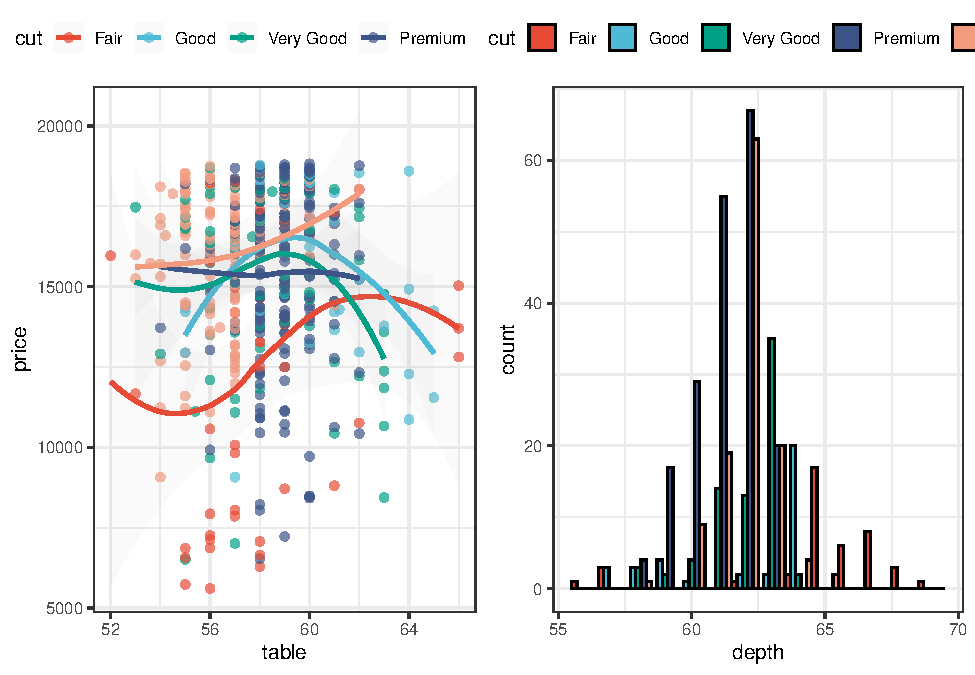
\includegraphics[width=0.8\linewidth]{/Users/robertjdellinger/Library/Mobile Documents/com~apple~CloudDocs/Documents/Applications/Github/template-repository/Output/Figures/Fig-data-visualization-plot-1} 

}

\caption{Example of a scatter plot}\label{fig:data-visualization-plot}
\end{figure}

\begin{Shaded}
\begin{Highlighting}[]
\CommentTok{\# Example of saving a plot}
\CommentTok{\# ggsave(filename = here(output\_path\_images, "plot\_name.png"), }
\CommentTok{\# plot = last\_plot(), width = 6, height = 4)}
\end{Highlighting}
\end{Shaded}

\section{Literature Cited}\label{literature-cited}

Citing the packages and data used in the analysis is important for
reproducibility and transparency. The following code generates a
bibliography of all loaded packages. Items can be cited directly within
the documentation using the syntax \texttt{@key} where key is the
citation key in the first line of the entry, e.g., R Core Team (2024),
Wickham et al. (2024), Wickham (2023), Müller (2020). To put citations
in parentheses, use \texttt{{[}@key{]}} instead.

\phantomsection\label{refs}
\begin{CSLReferences}{1}{0}
\bibitem[\citeproctext]{ref-R-here}
Müller, K. (2020). \emph{Here: A simpler way to find your files}.
\url{https://here.r-lib.org/}

\bibitem[\citeproctext]{ref-R-base}
R Core Team. (2024). \emph{R: A language and environment for statistical
computing}. R Foundation for Statistical Computing.
\url{https://www.R-project.org/}

\bibitem[\citeproctext]{ref-R-tidyverse}
Wickham, H. (2023). \emph{Tidyverse: Easily install and load the
tidyverse}. \url{https://tidyverse.tidyverse.org}

\bibitem[\citeproctext]{ref-R-ggplot2}
Wickham, H., Chang, W., Henry, L., Pedersen, T. L., Takahashi, K.,
Wilke, C., Woo, K., Yutani, H., Dunnington, D., \& van den Brand, T.
(2024). \emph{ggplot2: Create elegant data visualisations using the
grammar of graphics}. \url{https://ggplot2.tidyverse.org}

\end{CSLReferences}

\end{document}
